\documentclass[aps,prb,twocolumn,floatfix,nofootinbib,superscriptaddress]{revtex4-2}

\usepackage{amsmath,amssymb,amsthm,mathtools,bm}
\usepackage{booktabs}
\usepackage{graphicx}
\usepackage[colorlinks=true,linkcolor=blue,citecolor=blue,urlcolor=blue]{hyperref}
\usepackage{microtype}

\newcommand{\tr}{\operatorname{tr}}
\newcommand{\ii}{\mathrm{i}}
\newcommand{\code}[1]{\texttt{#1}}

\hypersetup{
  pdftitle={Pure-State Tangent Spectral Flow of a Frozen Adaptive-Circuit Record},
  pdfauthor={Asadullah Bhuiyan}
}

\begin{document}

\title{Pure-State Tangent Spectral Flow of a Frozen\
Adaptive-Circuit Record: CPU Pilot Protocol}
\author{Asadullah Bhuiyan}
\affiliation{Class-A fermionic adaptive-circuit project}
\date{September 3, 2026}

\begin{abstract}
We specify a CPU pilot that resolves the projective many-body singular gaps of
a trajectory-resolved adaptive Chern circuit as boundary flux is threaded.
For each of a soft explicit interface and a hard support-terminated wall, one
zero-flux Born trajectory is generated with a raster-$y$ measurement schedule
and then replayed at 17 static twists in each orientation.  The geometry is
$N_x\times N_y=16\times20$, the duration is 40 complete cycles, and all runs
use a pure half-filled initial state, $n_{\mathrm{shell}}=1$, perfect
correction, no postselection, and complex128 arithmetic.  The Gaussian
tangent cocycle is initialized in the exact occupied--empty decomposition of
the cycle-zero Slater determinant and accumulated without a burn-in reset over
the complete 40-cycle word.  Its one-leg singular values generate the
coherent one-particle--one-hole sector of the projectivized many-body singular
spectral singular spectrum.  We save up to 64 finite low-gap candidates,
require at least 32, and continuously follow 32 branches by their occupied-
and empty-leg overlaps.  Wall-resolved weights define a
spectral particle--hole excitation charge.  This quantity is neither a
fractional occupation of the evolving pure state nor a physical pumped charge,
and no quantization criterion is imposed.  This note fixes the protocol,
estimators, continuation rule, numerical checks, output contract, and claim
boundary.  New circuit results are intentionally deferred; the completed
equilibrium flattened-Hamiltonian pump is included only as calibration and
motivation.
\end{abstract}

\maketitle

\section{Question and claim boundary}

The class-A adaptive protocol measures localized overcomplete-Wannier (OW)
occupations and applies outcome-dependent fermionic feedback without
postselection~\cite{BhuiyanPanJian2026}.  For a fixed trajectory record
$\boldsymbol m$, the ordered many-body evolution operator (mEO) is denoted
$\hat V_{\boldsymbol m}$.  We ask whether its slow projective tangent sector
contains wall-localized modes whose spectral identity winds under a boundary
twist $\phi$.

This question differs from the equilibrium wall-charge pump.  In the latter,
one diagonalizes a static single-particle Hamiltonian, continuously transports
its occupied projector around a flux loop, and compares the regional charge of
that projector at the endpoints.  In the circuit, the physical pure-state
projector generated by independent static replays closes under a large gauge
transformation.  Continuing that projector therefore reproduces the static
closure already tested by the preceding pilot.  The present experiment instead
continues elementary one-particle--one-hole tangent modes of the normalized
trajectory map.

Accordingly, the pilot may establish a flux-dependent projective gap, wall
localization, branch exchange, and a signed \emph{spectral excitation charge}.
It cannot by itself establish an integer Hall pump, a current integrated over
monitored time, or a fractional occupation of a Lyapunov mode.  Neither an
integer excitation charge nor exact spectral closure is an acceptance gate.

\section{Completed equilibrium calibration}
\label{sec:equilibrium}

The prior equilibrium calculation provides the target phenomenon but not a
proof that the circuit tangent spectrum realizes it.  For OW trial family
$\nu=A,B$ and band $n=\pm$, it constructs
\begin{equation}
 F_{\nu n}(\phi)=\sum_{\bm R}
 |W_{\bm R,\nu n}(\phi)\rangle
 \langle W_{\bm R,\nu n}(\phi)|
\end{equation}
and the flattened one-body operator
\begin{equation}
 H_{\rm flat}(\phi)=F_{A+}+F_{B+}-F_{A-}-F_{B-}.
 \label{eq:hflat}
\end{equation}
The benchmark used $N_x\times N_y=20\times40$, $1600$ one-particle
orbitals, rank 800, $n_{\rm shell}=1$, $\alpha_{\rm top}=1$,
$\alpha_{\rm triv}=30$, and walls at $x=5,15$.  Both untruncated and
support-terminated OW constructions were tested.

Two state prescriptions answer different questions.  The instantaneous
projector occupies the globally lowest 800 eigenstates at every $\phi$; it is
the finite-size ground state and closes after $2\pi$.  The continued projector
chooses its occupied modes once at $\phi_0=\pm10^{-7}$ and matches them between
neighboring fluxes by maximum overlap.  A Hungarian assignment enforces a
one-to-one match, while an SVD polar rotation aligns clusters split by less
than $10^{-9}$.  Occupations are never reselected.  This produces a diabatic
continuation through the exponentially small wall anticrossing while
remaining adiabatic to the bulk.

For regional projectors $R_L,R_R$, the reported transferred charge is
\begin{equation}
 q_{\rm pump}=\frac12\left[\Delta\tr(R_RP)-\Delta\tr(R_LP)\right].
 \label{eq:equilibrium-pump}
\end{equation}
At $20\times40$ and $\phi_0=+10^{-7}$, the instantaneous result is
$1.49\times10^{-8}$ (untruncated) or $2.52\times10^{-9}$ (truncated),
whereas continued increasing flux gives $0.9839718573$ and $0.9808096958$.
The opposite winding gives $-0.9999999800$ and $-1.0000000032$.
Charge conservation is satisfied within $1.14\times10^{-13}$ and more than
$0.9999987$ of the transfer lies in a two-cell window around the physical
walls.  The noninteger $0.98$ endpoint is stable on 129, 257, and
endpoint-refined 751-point meshes: it reflects the regulated starting mode's
small weight on the opposite wall, not inadequate flux resolution.

\begin{figure}[t]
 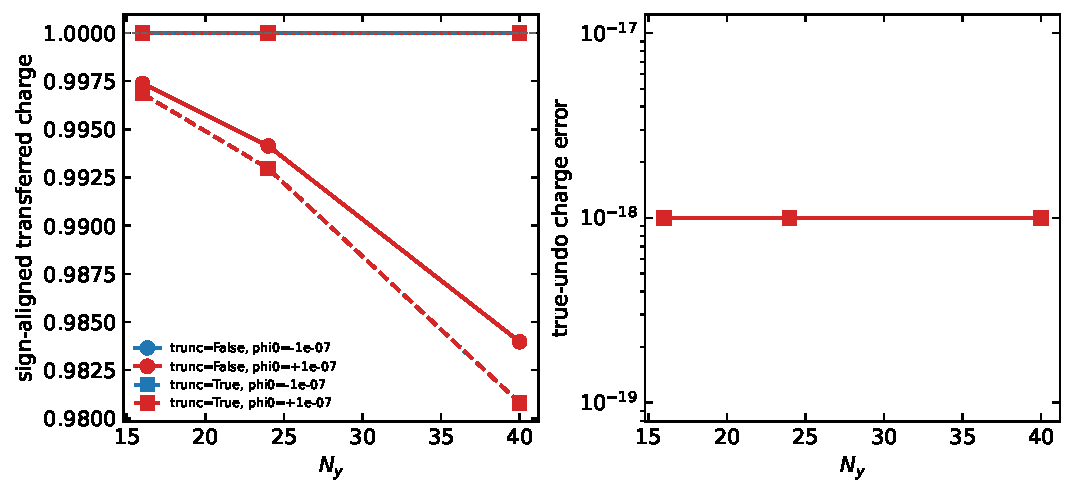
\includegraphics[width=\columnwidth]{../../../../notebooks/flattened_hamiltonian_analysis/outputs/exact_wall_charge_pump_reversibility_v1/run_20260901_162444/reversibility_and_offset_sensitivity.pdf}
 \caption{Completed equilibrium flattened-Hamiltonian calibration.  Left:
 sign-aligned continued wall-charge transfer for $N_y=16,24,40$, both OW wall
 constructions, and both signs of the $10^{-7}$ starting offset.  One winding
 is essentially integer; the partner reflects the initial opposite-wall
 weight.  Right: a true reverse traversal, initialized from the forward
 endpoint, undoes the transfer to $10^{-18}$-scale or better.  These are
 previously completed equilibrium results, not outputs of the present circuit
 pilot.}
 \label{fig:equilibrium-pump}
\end{figure}

The true undo follows the cached forward path backward from its endpoint.  For
$N_y=16,24,40$, both wall constructions and both offset signs obey
$q_{\rm undo}=-q_{\rm forward}$ to stored precision, with normalized projector
return error between $5.3\times10^{-22}$ and $4.2\times10^{-18}$; see
Fig.~\ref{fig:equilibrium-pump}.  This validates the continuation algorithm.
It does not make two independently initialized opposite windings literal time
reverses.

\begingroup
\sloppy
The quoted endpoint and mesh data are stored in
\path{notebooks/flattened_hamiltonian_analysis/outputs/exact_wall_charge_pump_refined_v1/run_20260901_002219/};
the size, offset, and true-undo audit and the plotted source are stored in
\path{notebooks/flattened_hamiltonian_analysis/outputs/exact_wall_charge_pump_reversibility_v1/run_20260901_162444/}.
Both directories contain machine-readable manifests and CSV tables in
addition to the displayed figure.
\endgroup

The circuit pilot deliberately does not transplant Eq.~\eqref{eq:equilibrium-pump}
onto its closing physical projector.  Instead it asks whether the low-gap
tangent excitations display an analogous exchange of wall character.  The
equilibrium result therefore fixes the comparison language and expected
spatial signature, while quantization remains outside the circuit acceptance
criteria.

\section{Locked circuit protocol}

\subsection{Geometry and dynamics}

Both wall constructions use the parameters in Table~\ref{tab:contract}.  A
cycle is a raster-$y$ ordered composition of OW-number measurements with
conditional fermionic swaps.  Distinct OW stabilizers need not commute, and
the raster convention is therefore part of the scientific definition of the
ordered word rather than a performance option.

\begin{table}[b]
\caption{Locked numerical contract.  The independent unit of computation is
one static twist replay of one immutable wall-specific record.}
\label{tab:contract}
\begin{ruledtabular}
\begin{tabular}{ll}
quantity & value \\
\hline
geometry & $N_x\times N_y=16\times20$ \\
physical cycles & $40=2N_y$ \\
OW support & $n_{\mathrm{shell}}=1$ \\
mass parameters & $\alpha_1=1$, $\alpha_2=30$ \\
domain interval & $x\in[4,12]$ \\
initial state & pure, half filled \\
measurement order & raster-$y$ \\
feedback & perfect correction \\
postselection & disabled \\
arithmetic & complex128 \\
twist points & $17$ per orientation \\
tangent window & cycles $1$--$40$ \\
saved candidates & up to $64$ finite; at least $32$ \\
continued branches & $32$
\end{tabular}
\end{ruledtabular}
\end{table}

The soft arm retains the OW tails throughout the cylinder and measures every
site.  The hard arm truncates the OW construction to the prescribed domain
and performs the canonical exterior preparation before measuring only the
active slab.  Each arm receives an independently generated zero-twist
reference because its active channel sequence and Born outcomes differ.

The earlier static-response campaign used random-serial records.  Those files
are retained as immutable provenance but are not replayed here.  Reordering a
saved stochastic word would define a different noncommuting circuit.  This
pilot therefore generates new raster-$y$ reference records in its own
versioned result directory.

\subsection{Frozen record and signed twist grid}

For each arm, a single zero-twist trajectory produces a cycle-zero correlation
matrix $G_0$, the final $G_{40}$, and the ordered record
$\boldsymbol m$.  A forced replay at zero twist must reproduce $G_{40}$ before
any flux task is admitted.  The same $G_0$ and the same outcomes, feedback
targets, and ordered site list are then imposed at every twist in both
orientations.

For $\sigma=+1$ (counterclockwise) and $\sigma=-1$ (clockwise),
\begin{equation}
 \phi_j^{(\sigma)}
 =-\sigma\,10^{-7}
 +\sigma\frac{2\pi j}{16},
 \qquad j=0,\ldots,16.
 \label{eq:twist-grid}
\end{equation}
The two sweeps therefore share the same exactly zero-twist stochastic word but
start on opposite sides of the potentially ambiguous crossing.  The
$10^{-7}$ regulator selects a reproducible side of that crossing while being
negligible on the scale of the flux step.  It can improve apparent branch
quantization by preventing a numerical eigensolver from making an arbitrary
choice inside a nearly degenerate subspace; it does not create topological
quantization and is not included as evidence for it.

The cycle-zero state is placed in the uniform gauge
\begin{equation}
 U_\phi=\exp\!\left(\ii\phi y/N_y\right),\qquad
 G_0(\phi)=U_\phi G_0 U_\phi^\dagger,
\end{equation}
and the OW modes are rebuilt at the same static $\phi$ before replaying
$\boldsymbol m$ for 40 cycles.

\section{Pure-state tangent spectrum}

\subsection{Projective one-particle--one-hole sector}

Let $P_\star$ denote the cycle-zero occupied projector of the pure Slater
determinant.  Choose orthonormal occupied vectors
$\{\lvert v_i\rangle\}$ and empty vectors
$\{\lvert u_a\rangle\}$.  A Hermitian tangent perturbation is generated by
the coherent one-particle--one-hole direction
\begin{equation}
 \delta G_{ai}
 =\lvert u_a\rangle\langle v_i\rvert
 +\lvert v_i\rangle\langle u_a\rvert.
 \label{eq:tangent-direction}
\end{equation}
For a trajectory-resolved Gaussian map, this Grassmannian tangent sector is
the coherent one-particle--one-hole sector of the projectivized many-body
singular spectrum~\cite{BhuiyanGaussianTransfer2026,BhuiyanNambuTangent2026}.
Exact gain, loss, and occupation projections may make the underlying transfer
word singular; the normalized tangent map nevertheless remains well defined
on its finite directions, with null directions recorded explicitly.

At the beginning of cycle one, the canonical CPU engine diagonalizes the pure
projector and initializes complete occupied and empty one-leg frames.  Every
realized rank-one channel acts on their concatenation.  At each completed
cycle the two blocks are QR-stabilized independently, and their triangular
factors are accumulated in separately scaled cores.  No alignment window or
accumulator reset is used: the resulting cocycle is the complete finite word
from cycle 1 through cycle 40.

Let $\ell_i^{\mathrm{occ}}$ and $\ell_a^{\mathrm{emp}}$ be the logarithms of
the final singular values of the oriented occupied and empty one-leg blocks.
More explicitly, if $K_{\rm occ}=KV_{\rm occ}$ and
$K_{\rm emp}=KU_{\rm emp}$ denote the restricted 40-cycle products, their
stabilized singular decompositions are
\begin{align}
 K_{\rm occ}&=V_{\rm out}\,e^{L_{\rm occ}}V_{\rm in}^\dagger,\\
 K_{\rm emp}&=U_{\rm out}\,e^{L_{\rm emp}}U_{\rm in}^\dagger.
 \label{eq:block-svd}
\end{align}
Thus $v_i$ is an output column of $V_{\rm out}$ and $u_a$ is an output
column of $U_{\rm out}$; the corresponding input columns are retained as
well.  Equivalently, these output columns diagonalize the two restricted
$KK^\dagger$ blocks.  They label coherent directions, not distinguishable
particles in the reference trajectory.
The repository convention forms the particle--hole tangent rate
\begin{equation}
 \lambda_{ai}
 =\frac{\ell_i^{\mathrm{occ}}+\ell_a^{\mathrm{emp}}}{40}.
 \label{eq:pair-rate}
\end{equation}
Equivalently, the empty-minus-occupied orientation is already absorbed into
the definition of the occupied one-leg block.  If the selected Slater ray is
dominant, the corresponding projective excitation gap of
\begin{equation}
 \hat H_{\mathrm{eff}}(\phi)
 =-\log\!\left[
 \hat V_{\boldsymbol m}(\phi)
 \hat V_{\boldsymbol m}^\dagger(\phi)
 \right]
\end{equation}
is
\begin{equation}
 \Delta E_{ai}=-2\bigl(
 \ell_i^{\mathrm{occ}}+\ell_a^{\mathrm{emp}}
 \bigr),\qquad
 \Delta\epsilon_{ai}=\frac{\Delta E_{ai}}{40}=-2\lambda_{ai}.
 \label{eq:effective-gap}
\end{equation}
These are gaps relative to the selected projective ray.  They do not determine
the additive zero of the absolute many-body spectrum.

\subsection{Candidate selection and spatial data}

All finite pairs are constructed before truncation.  Up to 64 candidates with
smallest $\lvert\lambda_{ai}\rvert$ are saved at each twist, and the exact
finite-pair and saved-candidate counts accompany every task.  At least 32 are
required because 32 branches are continued.  For every
candidate the output and input occupied and empty vectors, singular residual,
pair rate, effective gap, cell density, $x$ density, and wall weights are
retained.  Saving a pool twice as large as the reported branch set permits a
continued mode to move away from the instantaneous 32 lowest gaps near an
avoided crossing without being lost.

\section{Flux continuation and wall excitation charge}

\subsection{Common gauge and overlap assignment}

Spatial probabilities are gauge invariant, but eigenvector overlaps between
neighboring twists are not.  Before continuation, every input and output mode
is transformed back to the common zero-twist coordinate gauge by
$U_\phi^\dagger$.  Let $(v_i,u_a)$ and $(v_j',u_b')$ denote candidates at
neighboring twists.  Their matching score is
\begin{equation}
 \mathcal O_{ai,bj}
 =\bigl\lvert\langle v_i\vert v_j'\rangle\bigr\rvert
  \bigl\lvert\langle u_a\vert u_b'\rangle\bigr\rvert.
 \label{eq:mode-overlap}
\end{equation}
A rectangular linear assignment maps the 32 continued branches into up to 64
finite current candidates by maximizing the total overlap.  The run requires
at least 32 finite candidates at every flux; exact null directions are never
promoted into artificial modes merely to fill the table.  A $10^{-6}$-weighted gap
distance breaks only numerical ties.  Clockwise and counterclockwise branches
are continued independently from their respective regulated origins.  Step
overlaps and endpoint closure overlaps are diagnostics and remain in the raw
analysis product.

\subsection{What ``mode occupation'' means}

For a pure trajectory the state occupations of the two one-leg sectors are
exactly one and zero.  The nontrivial flux-dependent observables are their
regional probability weights.  With $R_L$ and $R_R$ the disjoint Voronoi
basins of the walls at $x=4$ and $x=12$, define
\begin{align}
 p_{L/R}^{\mathrm{occ}}(\phi)
 &=\langle v_i(\phi)\rvert R_{L/R}\lvert v_i(\phi)\rangle,\\
 p_{L/R}^{\mathrm{emp}}(\phi)
 &=\langle u_a(\phi)\rvert R_{L/R}\lvert u_a(\phi)\rangle.
\end{align}
The excitation projector obtained by removing $v_i$ and adding $u_a$ is
\begin{equation}
 P_{ai}=P_\star-lvert v_i\rangle\langle v_i\rvert
                   +lvert u_a\rangle\langle u_a\rvert.
\end{equation}
Its normalized left--right excitation charge is
\begin{equation}
 q_{ai}(\phi)=\frac12\left[
 (p_R^{\mathrm{emp}}-p_L^{\mathrm{emp}})
 -(p_R^{\mathrm{occ}}-p_L^{\mathrm{occ}})
 \right].
 \label{eq:excitation-charge}
\end{equation}
Thus $q_{ai}\simeq+1$ places the added particle on the right wall and the hole
on the left, while $q_{ai}\simeq-1$ reverses that assignment.  A value near
zero can mean same-wall support or delocalization; the four underlying weights
are therefore always saved and must be inspected with $q_{ai}$.

The labels ``occupied'' and ``empty'' refer first to the cycle-zero sectors
from which the tangent legs originate.  To test their endpoint interpretation
rather than assume it, the data product also stores
$\langle v_i|P_T|v_i\rangle$, $\langle u_a|P_T|u_a\rangle$ and the projector
residuals $\|P_Tv_i-v_i\|$ and $\|P_Tu_a\|$ after undoing the common flux
gauge.  These diagnostics state directly whether a reported output leg is
occupied-like or empty-like in the final physical Slater determinant.

Equation~\eqref{eq:excitation-charge} is a property of a derived spectral
excitation.  It is not the total charge transported by the monitored state.
For comparison only, every replay also saves the final physical
$N_L$, $N_R$, and $N_{\mathrm{tot}}$ used in the preceding static-response
pilot.

\section{Numerical validation and data contract}

The physical evolution always calls the canonical CPU entry point
\code{classA\_U1FGTN.run\_markov\_circuit}.  Tangent tracking is an opt-in
engine mode and does not duplicate or replace the Markov cycle loop.  The CPU
occupied--empty implementation is tested against the canonical GPU block
convention on small pure systems and against a direct full-product Gram
reconstruction.

Before production, the following checks are mandatory:
\begin{enumerate}
  \item each raster-$y$ reference has a valid result/completion pair;
  \item a forced zero-twist replay reproduces the sampled final correlation
        matrix to normalized Frobenius error below $10^{-12}$;
  \item all physical and tangent arrays are complex128 or float64 as
        appropriate;
  \item charge continuity agrees with the integer feedback source to
        $10^{-9}$;
  \item tangent branch probabilities are finite and no invalid branch is
        admitted;
  \item selected singular-vector residuals remain below $10^{-8}$;
  \item tangent observation leaves the physical final state unchanged on a
        common-seed regression.
\end{enumerate}

There are $2\times2\times17=68$ independent twist tasks.  Each writes one
compressed NPZ followed by one completion JSON containing the task identity,
configuration identity, reference hash, filename, byte count, and SHA-256.
A restart skips a task only after both files verify.  Missing, partial, or
mismatched pairs are recomputed.  The completed random-serial campaign remains
untouched; the present products live under
\code{results/N16x20\_frozen\_flux\_pure\_tangent\_v1}.

The analysis product contains the continued 32-branch arrays, a flat CSV, and
a JSON ledger of overlap and residual diagnostics.  No acceptance field tests
$q_{ai}$ against an integer and no result is promoted to a pump invariant.

\section{Execution}

The production job uses 28 independent processes on physical CPU cores
28--55, with one BLAS thread per process.  A single parent progress bar reports
verified and completed twist points.  The tmux session is named
\code{frozen\_flux\_pure\_tangent\_N16x20\_v1}; its persistent log and all
scientific products reside in the versioned result directory.  One hard and
one soft task are first executed in a separate smoke directory.  The branch
analysis runs only after all 68 result/completion pairs verify.

\section{Deferred interpretation}

No numerical conclusion is part of this protocol document.  A subsequent
results amendment may discuss whether low-gap branches remain localized,
exchange wall character, show orientation-dependent monodromy, or correlate
with the static conditioned charge response.  Such an amendment must retain
the distinction among an equilibrium occupied-projector pump, a
trajectory-conditioned static replay, a pure-state tangent excitation, and a
physical time-dependent monitored pump.

\bibliographystyle{apsrev4-2}
\bibliography{references}

\end{document}
